\subsection{Fase di progettazione di dettaglio e codifica}

\subsubsection{Incremento I}

I dati riportati di seguito si riferiscono al periodo che va dal 08-03-2021 al 10-03-2021.

\begin{minipage}[b]{0.65\linewidth}
\begin{small}

\begin{longtable}{ c | c c c c c c | c} 
 \rowcolor{coloreRosso}
 \color{white}{\textbf{Nominativo}} &
 \color{white}{\textbf{RE}} &
 \color{white}{\textbf{AM}} &
 \color{white}{\textbf{AN}} &
 \color{white}{\textbf{PT}} &
 \color{white}{\textbf{PR}} &
 \color{white}{\textbf{VE}} &
 \color{white}{\textbf{Tot.}} \\
 	
 \BM{} & - & 2 & - & 2 & - & - & 4 \\ 
 \PA{} & - & - & - & - & 2 & 2 & 4 \\ 
 \RA{} & - & - & - & 3 & - & 2 & 5\\ 
 \SH{} & - & - & - & 1 & - & 3 & 4 \\ 
 \SG{} & - & - & - & 1 & 2 & 2 & 5 \\ 
 \SP{} & 2 & - & - & - & - & 2 & 4 \\ 
 \ZM{} & - & - & - & 3 & - & 3 & 6 \\
 
 	\rowcolor{coloreRosso}
 	\color{white}{\textbf{Totale ore ruolo}} &
 	\color{white}{\textbf{2}} &
 	\color{white}{\textbf{2}} &
 	\color{white}{\textbf{-}} &
 	\color{white}{\textbf{10}} &
 	\color{white}{\textbf{4}} &
 	\color{white}{\textbf{14}} &
 	\color{white}{\textbf{32}} \\
	\rowcolor{white}
	\captionsetup{width=.9\textwidth}
 	\caption{Distribuzione delle ore nel pri IIIIII di progettazione architetturale}
\end{longtable}

\end{small}
\end{minipage}
\begin{minipage}[b]{.3\linewidth}
\begin{small}

\begin{longtable}{ c | c | c} 
 	\rowcolor{coloreRosso}
 	\color{white}{\textbf{Ruolo}} &
 	\color{white}{\textbf{Ore}} &
 	\color{white}{\textbf{Costo €}} \\
 	
 	Responsabile & 2 & 60\\
 	Amministratore & 2 & 40\\
 	Analista & - & -\\
 	Progettista & 10 & 220\\
 	Programmatore & 4 & 60\\
 	Verificatore & 14 & 210\\
 	
 	\rowcolor{coloreRosso}
 	\color{white}{\textbf{Totale}} &
 	\color{white}{\textbf{32}} &
 	\color{white}{\textbf{590}}\\
 	\rowcolor{white}
 	\caption{Costi per ruolo nel primo periodo di progettazione architetturale}
\end{longtable}

\end{small}
\end{minipage}

\begin{figure}[!htb]   
    \centering
    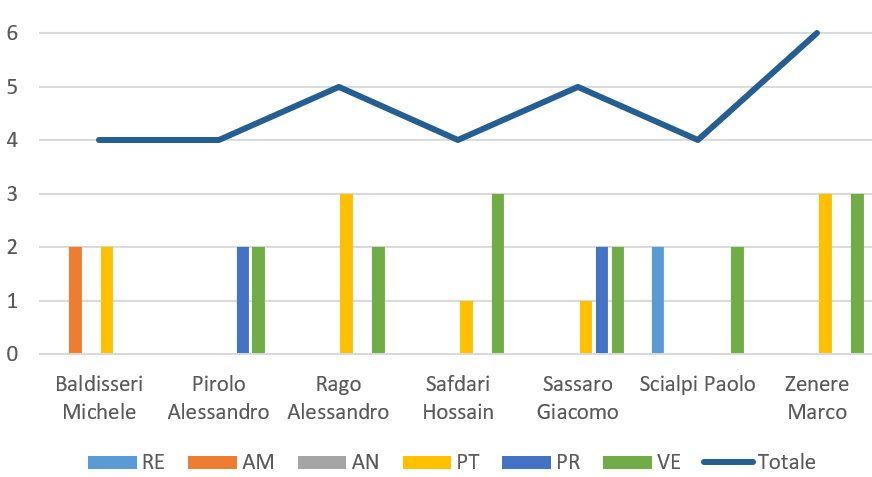
\includegraphics[width=0.85\textwidth]{Images/inc1}
	\caption{Ripartizione oraria per ciascun membro durante l'incremento I}
\end{figure}





\subsubsection{Incremento II}

I dati riportati di seguito si riferiscono al periodo che va dall' 10-03-2021 al 12-03-2021.

\begin{minipage}[b]{0.65\linewidth}
\begin{small}

\begin{longtable}{ c | c c c c c c | c} 
 \rowcolor{coloreRosso}
 \color{white}{\textbf{Nominativo}} &
 \color{white}{\textbf{RE}} &
 \color{white}{\textbf{AM}} &
 \color{white}{\textbf{AN}} &
 \color{white}{\textbf{PT}} &
 \color{white}{\textbf{PR}} &
 \color{white}{\textbf{VE}} &
 \color{white}{\textbf{Tot.}} \\
 	
 \BM{} & - & 3 & - & 4 & - & - & 7 \\ 
 \PA{} & - & - & - & 5 & 1 & - & 6 \\ 
 \RA{} & - & - & - & 2 & - & 3 & 5\\ 
 \SH{} & - & - & - & 6 & - & - & 6 \\ 
 \SG{} & - & - & - & 5 & - & - & 5 \\ 
 \SP{} & - & - & - & - & 7 & - & 7 \\ 
 \ZM{} & 1 & - & - & - & 5 & - & 6 \\
 
 	\rowcolor{coloreRosso}
 	\color{white}{\textbf{Totale ore ruolo}} &
 	\color{white}{\textbf{1}} &
 	\color{white}{\textbf{3}} &
 	\color{white}{\textbf{-}} &
 	\color{white}{\textbf{22}} &
 	\color{white}{\textbf{13}} &
 	\color{white}{\textbf{3}} &
 	\color{white}{\textbf{42}} \\
	\rowcolor{white}
	\captionsetup{width=.9\textwidth}
 	\caption{Distribuzione delle ore nel periodo II della Progettazione architetturale}
\end{longtable}

\end{small}
\end{minipage}
\begin{minipage}[b]{.3\linewidth}
\begin{small}

\begin{longtable}{ c | c | c} 
 	\rowcolor{coloreRosso}
 	\color{white}{\textbf{Ruolo}} &
 	\color{white}{\textbf{Ore}} &
 	\color{white}{\textbf{Costo €}} \\
 	
 	Responsabile & 1 & 30\\
 	Amministratore & 3 & 60\\
 	Analista & - & -\\
 	Progettista & 22 & 484\\
 	Programmatore & 13 & 195\\
 	Verificatore & 3 & 45\\
 	
 	\rowcolor{coloreRosso}
 	\color{white}{\textbf{Totale}} &
 	\color{white}{\textbf{42}} &
 	\color{white}{\textbf{814}}\\
 	\rowcolor{white}
 	\caption{Costi per ruolo nel periodo II della Progettazione architetturale}
\end{longtable}

\end{small}
\end{minipage}

\begin{figure}[!htb]   
    \centering
    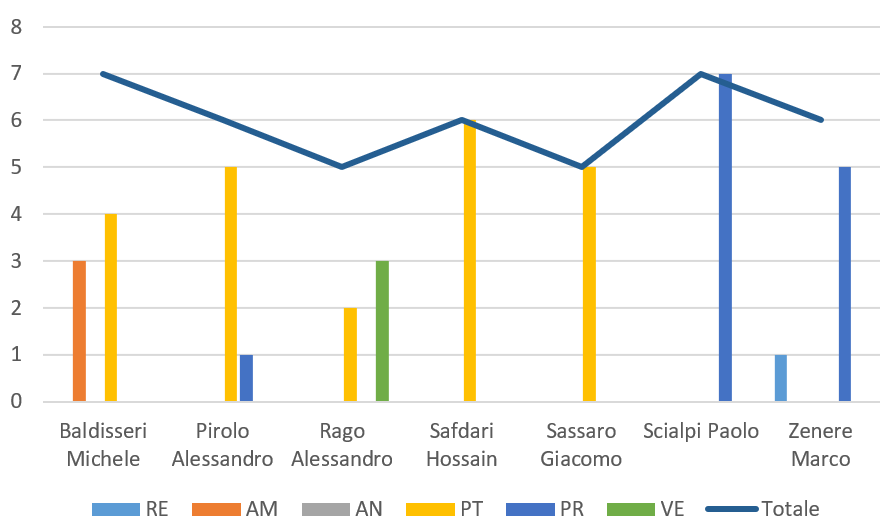
\includegraphics[width=0.9\textwidth]{Images/inc2}
	\caption{Ripartizione oraria per ciascun membro durante l'incremento II}
\end{figure}

\subsubsection{Incremento III}

I dati riportati di seguito si riferiscono al periodo che va dal 12-03-2021 al 16-03-2021.

\begin{minipage}[b]{0.65\linewidth}
\begin{small}

\begin{longtable}{ c | c c c c c c | c} 
 \rowcolor{coloreRosso}
 \color{white}{\textbf{Nominativo}} &
 \color{white}{\textbf{RE}} &
 \color{white}{\textbf{AM}} &
 \color{white}{\textbf{AN}} &
 \color{white}{\textbf{PT}} &
 \color{white}{\textbf{PR}} &
 \color{white}{\textbf{VE}} &
 \color{white}{\textbf{Tot.}} \\
 	
 \BM{} & - & - & - & 5 & 5 & - & 10 \\ 
 \PA{} & - & 2 & - & 5 & - & 3 & 10 \\ 
 \RA{} & - & - & - & 2 & 6 & - & 8\\ 
 \SH{} & 2 & - & - & 1 & 5 & - & 8 \\ 
 \SG{} & - & 4 & - & 5 & - & - & 9 \\ 
 \SP{} & - & - & - & 5 & 4 & - & 9 \\ 
 \ZM{} & 1 & - & - & - & 9 & - & 10 \\
 
 	\rowcolor{coloreRosso}
 	\color{white}{\textbf{Totale ore ruolo}} &
 	\color{white}{\textbf{3}} &
 	\color{white}{\textbf{6}} &
 	\color{white}{\textbf{-}} &
 	\color{white}{\textbf{23}} &
 	\color{white}{\textbf{29}} &
 	\color{white}{\textbf{3}} &
 	\color{white}{\textbf{64}} \\
	\rowcolor{white}
	\captionsetup{width=.9\textwidth}
 	\caption{Distribuzione delle ore nel periodo III della Progettazione architetturale}
\end{longtable}

\end{small}
\end{minipage}
\begin{minipage}[b]{.3\linewidth}
\begin{small}

\begin{longtable}{ c | c | c} 
 	\rowcolor{coloreRosso}
 	\color{white}{\textbf{Ruolo}} &
 	\color{white}{\textbf{Ore}} &
 	\color{white}{\textbf{Costo €}} \\
 	
 	Responsabile & 3 & 90\\
 	Amministratore & 6 & 120\\
 	Analista & - & -\\
 	Progettista & 23 & 506\\
 	Programmatore & 29 & 435\\
 	Verificatore & 3 & 45\\
 	
 	\rowcolor{coloreRosso}
 	\color{white}{\textbf{Totale}} &
 	\color{white}{\textbf{64}} &
 	\color{white}{\textbf{1196}}\\
 	\rowcolor{white}
 	\caption{Costi per ruolo nel periodo III della Progettazione architetturale}
\end{longtable}

\end{small}
\end{minipage}

\begin{figure}[!htb]   
    \centering
    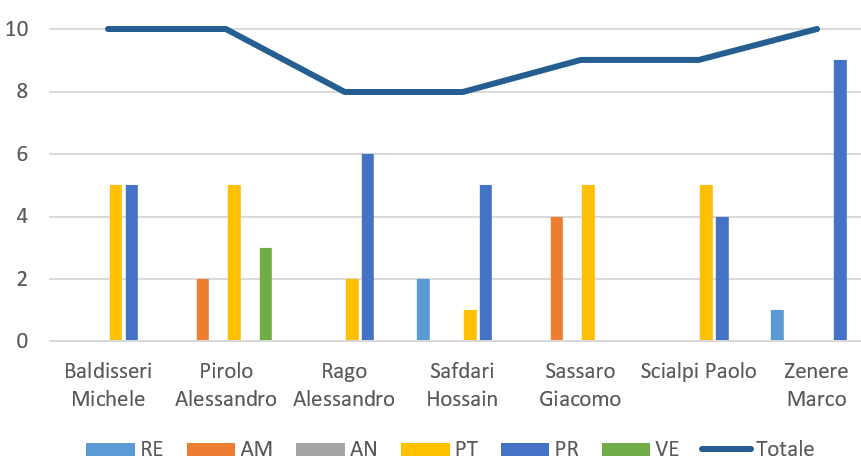
\includegraphics[width=0.9\textwidth]{Images/inc3}
	\caption{Ripartizione oraria per ciascun membro durante l'incremento III}
\end{figure}

\subsubsection{Incremento IV}

I dati riportati di seguito si riferiscono al periodo che va dal 16-03-2021 al 20-03-2021.

\begin{minipage}[b]{0.65\linewidth}
\begin{small}

\begin{longtable}{ c | c c c c c c | c} 
 \rowcolor{coloreRosso}
 \color{white}{\textbf{Nominativo}} &
 \color{white}{\textbf{RE}} &
 \color{white}{\textbf{AM}} &
 \color{white}{\textbf{AN}} &
 \color{white}{\textbf{PT}} &
 \color{white}{\textbf{PR}} &
 \color{white}{\textbf{VE}} &
 \color{white}{\textbf{Tot.}} \\
 	
 \BM{} & - & - & - & - & 9 & - & 9 \\ 
 \PA{} & - & 2 & - & - & 5 & - & 7 \\ 
 \RA{} & - & - & - & 5 & - & 4 & 9\\ 
 \SH{} & 2 & - & - & - & 5 & 2 & 9 \\ 
 \SG{} & - & - & - & 2 & 6 & - & 8 \\ 
 \SP{} & - & 3 & - & 2 & 2 & - & 7 \\ 
 \ZM{} & - & - & - & 2 & 2 & 4 & 8 \\
 
 	\rowcolor{coloreRosso}
 	\color{white}{\textbf{Totale ore ruolo}} &
 	\color{white}{\textbf{2}} &
 	\color{white}{\textbf{5}} &
 	\color{white}{\textbf{-}} &
 	\color{white}{\textbf{11}} &
 	\color{white}{\textbf{29}} &
 	\color{white}{\textbf{10}} &
 	\color{white}{\textbf{57}} \\
	\rowcolor{white}
	\captionsetup{width=.9\textwidth}
 	\caption{Distribuzione delle ore nel periodo III della Progettazione architetturale}
\end{longtable}

\end{small}
\end{minipage}
\begin{minipage}[b]{.3\linewidth}
\begin{small}

\begin{longtable}{ c | c | c} 
 	\rowcolor{coloreRosso}
 	\color{white}{\textbf{Ruolo}} &
 	\color{white}{\textbf{Ore}} &
 	\color{white}{\textbf{Costo €}} \\
 	
 	Responsabile & 2 & 60\\
 	Amministratore & 5 & 100\\
 	Analista & - & -\\
 	Progettista & 11 & 242\\
 	Programmatore & 29 & 435\\
 	Verificatore & 10 & 150\\
 	
 	\rowcolor{coloreRosso}
 	\color{white}{\textbf{Totale}} &
 	\color{white}{\textbf{57}} &
 	\color{white}{\textbf{987}}\\
 	\rowcolor{white}
 	\caption{Costi per ruolo nel periodo III della Progettazione architetturale}
\end{longtable}

\end{small}
\end{minipage}

\begin{figure}[!htb]   
    \centering
    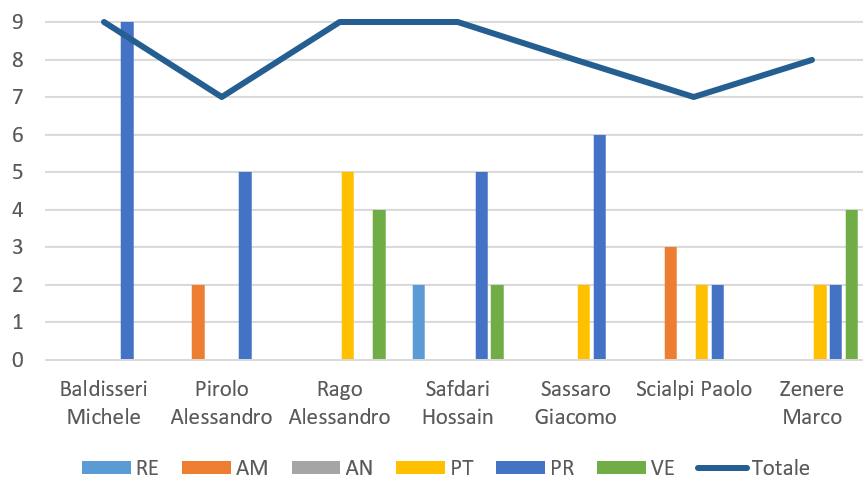
\includegraphics[width=0.9\textwidth]{Images/inc4}
	\caption{Ripartizione oraria per ciascun membro durante l'incremento IV}
\end{figure}

\subsubsection{Incremento V}

I dati riportati di seguito si riferiscono al periodo che va dal 20-03-2021 al 25-03-2021.

\begin{minipage}[b]{0.65\linewidth}
\begin{small}

\begin{longtable}{ c | c c c c c c | c} 
 \rowcolor{coloreRosso}
 \color{white}{\textbf{Nominativo}} &
 \color{white}{\textbf{RE}} &
 \color{white}{\textbf{AM}} &
 \color{white}{\textbf{AN}} &
 \color{white}{\textbf{PT}} &
 \color{white}{\textbf{PR}} &
 \color{white}{\textbf{VE}} &
 \color{white}{\textbf{Tot.}} \\
 	
 \BM{} & - & - & - & - & 5 & 3 & 8 \\ 
 \PA{} & - & - & - & - & 8 & - & 8 \\ 
 \RA{} & 4 & - & - & - & 2 & 1 & 7\\ 
 \SH{} & 2 & 3 & - & - & 3 & - & 8 \\ 
 \SG{} & - & - & - & - & 6 & - & 6 \\ 
 \SP{} & - & - & - & - & 2 & 4 & 6 \\ 
 \ZM{} & - & 3 & - & 4 & - & - & 7 \\
 
 	\rowcolor{coloreRosso}
 	\color{white}{\textbf{Totale ore ruolo}} &
 	\color{white}{\textbf{6}} &
 	\color{white}{\textbf{6}} &
 	\color{white}{\textbf{-}} &
 	\color{white}{\textbf{4}} &
 	\color{white}{\textbf{26}} &
 	\color{white}{\textbf{8}} &
 	\color{white}{\textbf{50}} \\
	\rowcolor{white}
	\captionsetup{width=.9\textwidth}
 	\caption{Distribuzione delle ore nel periodo III della Progettazione architetturale}
\end{longtable}

\end{small}
\end{minipage}
\begin{minipage}[b]{.3\linewidth}
\begin{small}

\begin{longtable}{ c | c | c} 
 	\rowcolor{coloreRosso}
 	\color{white}{\textbf{Ruolo}} &
 	\color{white}{\textbf{Ore}} &
 	\color{white}{\textbf{Costo €}} \\
 	
 	Responsabile & 6 & 180\\
 	Amministratore & 6 & 120\\
 	Analista & - & -\\
 	Progettista & 4 & 88\\
 	Programmatore & 26 & 390\\
 	Verificatore & 8 & 120\\
 	
 	\rowcolor{coloreRosso}
 	\color{white}{\textbf{Totale}} &
 	\color{white}{\textbf{50}} &
 	\color{white}{\textbf{898}}\\
 	\rowcolor{white}
 	\caption{Costi per ruolo nel periodo III della Progettazione architetturale}
\end{longtable}

\end{small}
\end{minipage}

\begin{figure}[!htb]   
    \centering
    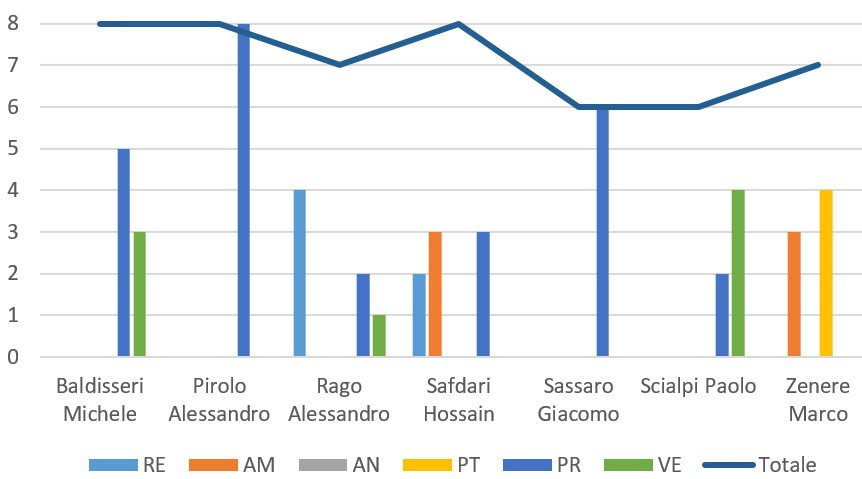
\includegraphics[width=0.9\textwidth]{Images/inc5}
	\caption{Ripartizione oraria per ciascun membro durante l'incremento V}
\end{figure}

\subsubsection{Incremento VI}

I dati riportati di seguito si riferiscono al periodo che va dal 25-03-2021 al 30-03-2021.

\begin{minipage}[b]{0.65\linewidth}
\begin{small}

\begin{longtable}{ c | c c c c c c | c} 
 \rowcolor{coloreRosso}
 \color{white}{\textbf{Nominativo}} &
 \color{white}{\textbf{RE}} &
 \color{white}{\textbf{AM}} &
 \color{white}{\textbf{AN}} &
 \color{white}{\textbf{PT}} &
 \color{white}{\textbf{PR}} &
 \color{white}{\textbf{VE}} &
 \color{white}{\textbf{Tot.}} \\
 	
 \BM{} & - & - & - & - & 2 & 4 & 6 \\ 
 \PA{} & - & - & - & - & 5 & 4 & 9 \\ 
 \RA{} & - & - & - & 3 & 5 & - & 8\\ 
 \SH{} & - & - & - & - & 6 & 2 & 8 \\ 
 \SG{} & - & 2 & - & - & 5 & 2 & 9 \\ 
 \SP{} & 2 & - & - & 2 & 4 & - & 8 \\ 
 \ZM{} & 1 & 1 & - & - & 5 & - & 7 \\
 
 	\rowcolor{coloreRosso}
 	\color{white}{\textbf{Totale ore ruolo}} &
 	\color{white}{\textbf{3}} &
 	\color{white}{\textbf{3}} &
 	\color{white}{\textbf{-}} &
 	\color{white}{\textbf{5}} &
 	\color{white}{\textbf{32}} &
 	\color{white}{\textbf{12}} &
 	\color{white}{\textbf{55}} \\
	\rowcolor{white}
	\captionsetup{width=.9\textwidth}
 	\caption{Distribuzione delle ore nel periodo III della Progettazione architetturale}
\end{longtable}

\end{small}
\end{minipage}
\begin{minipage}[b]{.3\linewidth}
\begin{small}

\begin{longtable}{ c | c | c} 
 	\rowcolor{coloreRosso}
 	\color{white}{\textbf{Ruolo}} &
 	\color{white}{\textbf{Ore}} &
 	\color{white}{\textbf{Costo €}} \\
 	
 	Responsabile & 3 & 90\\
 	Amministratore & 3 & 60\\
 	Analista & - & -\\
 	Progettista & 5 & 110\\
 	Programmatore & 32 & 480\\
 	Verificatore & 12 & 180\\
 	
 	\rowcolor{coloreRosso}
 	\color{white}{\textbf{Totale}} &
 	\color{white}{\textbf{55}} &
 	\color{white}{\textbf{920}}\\
 	\rowcolor{white}
 	\caption{Costi per ruolo nel periodo III della Progettazione architetturale}
\end{longtable}

\end{small}
\end{minipage}

\begin{figure}[!htb]   
    \centering
    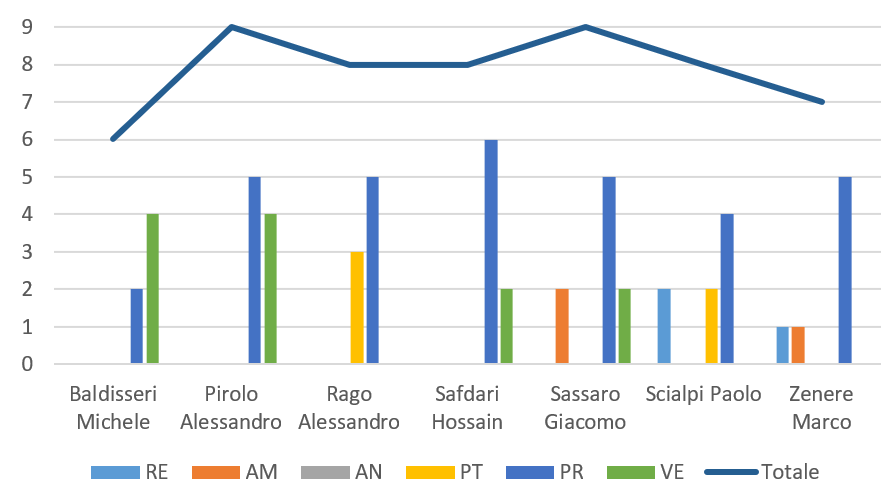
\includegraphics[width=0.9\textwidth]{Images/inc6}
	\caption{Ripartizione oraria per ciascun membro durante l'incremento VI}
\end{figure}

\subsubsection{Incremento VII}

I dati riportati di seguito si riferiscono al periodo che va dal 30-03-2021 al 02-04-2021.

\begin{minipage}[b]{0.65\linewidth}
\begin{small}

\begin{longtable}{ c | c c c c c c | c} 
 \rowcolor{coloreRosso}
 \color{white}{\textbf{Nominativo}} &
 \color{white}{\textbf{RE}} &
 \color{white}{\textbf{AM}} &
 \color{white}{\textbf{AN}} &
 \color{white}{\textbf{PT}} &
 \color{white}{\textbf{PR}} &
 \color{white}{\textbf{VE}} &
 \color{white}{\textbf{Tot.}} \\
 	
 \BM{} & - & 2 & - & - & - & 6 & 6 \\ 
 \PA{} & - & - & - & - & 2 & 6 & 8 \\ 
 \RA{} & - & - & - & - & 6 & - & 6\\ 
 \SH{} & - & - & - & - & 2 & 5 & 7 \\ 
 \SG{} & - & - & - & - & 2 & 6 & 8 \\ 
 \SP{} & - & 2 & - & - & 2 & 5 & 9 \\ 
 \ZM{} & 3 & - & - & - & - & 3 & 6 \\
 
 	\rowcolor{coloreRosso}
 	\color{white}{\textbf{Totale ore ruolo}} &
 	\color{white}{\textbf{3}} &
 	\color{white}{\textbf{2}} &
 	\color{white}{\textbf{-}} &
 	\color{white}{\textbf{-}} &
 	\color{white}{\textbf{14}} &
 	\color{white}{\textbf{31}} &
 	\color{white}{\textbf{50}} \\
	\rowcolor{white}
	\captionsetup{width=.9\textwidth}
 	\caption{Distribuzione delle ore nel periodo III della Progettazione architetturale}
\end{longtable}

\end{small}
\end{minipage}
\begin{minipage}[b]{.3\linewidth}
\begin{small}

\begin{longtable}{ c | c | c} 
 	\rowcolor{coloreRosso}
 	\color{white}{\textbf{Ruolo}} &
 	\color{white}{\textbf{Ore}} &
 	\color{white}{\textbf{Costo €}} \\
 	
 	Responsabile & 3 & 90\\
 	Amministratore & 2 & 40\\
 	Analista & - & -\\
 	Progettista & - & -\\
 	Programmatore & 14 & 210\\
 	Verificatore & 31 & 465\\
 	
 	\rowcolor{coloreRosso}
 	\color{white}{\textbf{Totale}} &
 	\color{white}{\textbf{50}} &
 	\color{white}{\textbf{805}}\\
 	\rowcolor{white}
 	\caption{Costi per ruolo nel periodo III della Progettazione architetturale}
\end{longtable}

\end{small}
\end{minipage}

\begin{figure}[!htb]   
    \centering
    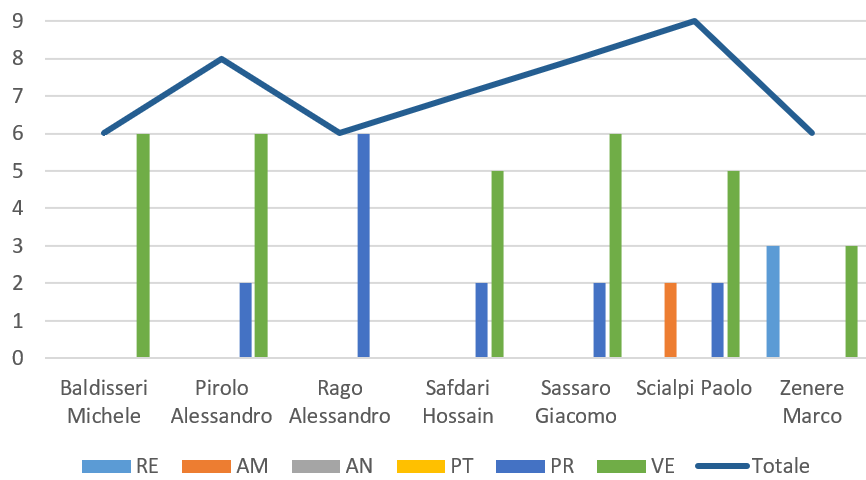
\includegraphics[width=0.9\textwidth]{Images/inc7}
	\caption{Ripartizione oraria per ciascun membro durante l'incremento VII}
\end{figure}

\subsubsection{Riepilogo}

\begin{minipage}[b]{0.65\linewidth}
\begin{small}

\begin{longtable}{ c | c c c c c c | c} 
 \rowcolor{coloreRosso}
 \color{white}{\textbf{Nominativo}} &
 \color{white}{\textbf{RE}} &
 \color{white}{\textbf{AM}} &
 \color{white}{\textbf{AN}} &
 \color{white}{\textbf{PT}} &
 \color{white}{\textbf{PR}} &
 \color{white}{\textbf{VE}} &
 \color{white}{\textbf{Tot.}} \\
 	
 \BM{} & - & 5 & - & 11 & 21 & 13 & 50 \\ 
 \SG{} & - & 6 & - & 13 & 21 & 10 & 50 \\ 
 \SH{} & 6 & 3 & - & 8 & 21 & 12 & 50 \\ 
 \PA{} & - & 4 & - & 10 & 21 & 15 & 50 \\ 
 \SP{} & 4 & 5 & - & 9 & 21 & 11 & 50 \\ 
 \RA{} & 4 & - & - & 15 & 21 & 10 & 50 \\ 
 \ZM{} & 6 & 4 & - & 9 & 21 & 10 & 50 \\
 
 \rowcolor{coloreRosso}
 	\color{white}{\textbf{Totale ore ruolo}} &
 	\color{white}{\textbf{20}} &
 	\color{white}{\textbf{27}} &
 	\color{white}{\textbf{-}} &
 	\color{white}{\textbf{75}} &
 	\color{white}{\textbf{147}} &
 	\color{white}{\textbf{81}} &
 	\color{white}{\textbf{350}} \\
 \rowcolor{white}
 \captionsetup{width=.9\textwidth}
 \caption{Distribuizione delle ore nel periodo di Progettazione di dettaglio e Codifica}
\end{longtable}

\end{small}
\end{minipage}
\begin{minipage}[b]{.3\linewidth}
\begin{small}

\begin{longtable}{ c | c | c} 
 	\rowcolor{coloreRosso}
 	\color{white}{\textbf{Ruolo}} &
 	\color{white}{\textbf{Ore}} &
 	\color{white}{\textbf{Costo €}} \\
 	
 	Responsabile & 20 & 600\\
 	Amministratore & 27 & 540\\
 	Analista & - & -\\
 	Progettista & 75 & 1650\\
 	Programmatore & 147 & 2205\\
 	Verificatore & 81 & 1215\\
 	
 	\rowcolor{coloreRosso}
 	\color{white}{\textbf{Totale}} &
 	\color{white}{\textbf{350}} &
 	\color{white}{\textbf{6210}}\\
 	\rowcolor{white}
 	\caption{Costi per ruolo nel periodo di Prog. di dettaglio e Codifica}
\end{longtable}

\end{small}
\end{minipage}

I seguenti grafici riassumo i dati ottenuti.

\begin{figure}[!htb]
   \begin{minipage}{0.6\textwidth}
     \centering
     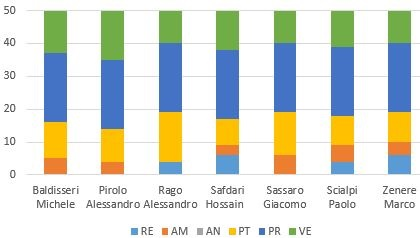
\includegraphics{Images/PO-Codifica}
     \caption{Ripartizione oraria per ciascun membro nella fase di Prog. di dettaglio e Codifica}
   \end{minipage}\hspace{0.1\textwidth}
   \begin{minipage}{0.3\textwidth}
     \centering
     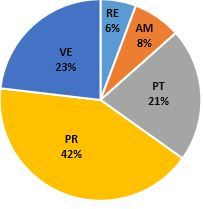
\includegraphics[width=.9\textwidth]{Images/PE-Codifica}
     \captionsetup{width=.9\textwidth}
     \caption{Ripartizione ore totali nella fase di Prog. di dettaglio e Codifica}
   \end{minipage}
\end{figure}

\newpage